\chapter{Performance and Limitations of FIDSs\label{chap:app}}

\section{Introduction\label{sec:app.intro}}

In the previous chapters, we have discussed the perspectives offered by applying \gls{fl} to \glspl{ids}, notably in terms of collaboration.
Based on the insights gained from the literature, it is now clear that \gls{fl} can be used to train a global model over the distributed data of a federation of organizations.
It even seems that \gls{fl} could be used to share attack knowledge, still without sharing participants' local data.

In this chapter, we present critical examples showing the challenges that arise when applying \gls{fl} to \glspl{cids}.
We start by laying out in \Cref{sec:app.overview} the practical use case that will be used throughout the rest of the manuscript.
Then, we highlight some limitations of \gls{fl} in the context of \glspl{cids} in \Cref{sec:app.demo}, based on our demonstration paper published at ICDCS 2024~\cite{lavaur_icdcs_demo_2024}.
%In the last sections, we further analyze some of the results, using the insights gained from the work of Akshat Chaudhary, an intern that worked on this project in 2023. -- TODO

\begin{highlightbox}{Contributions of this chapter}
  \begin{itemize}[\textbullet, leftmargin=*, labelsep=10pt]
    \item A practical use case for \gls{fl} in the context of \glspl{cids} involving multiple organizations.
    \item A demonstration of the limitations of \gls{fl} in the context of \glspl{cids}, notably in terms of data heterogeneity and susceptibility to poisoning attacks.
  \end{itemize}
\end{highlightbox}



% --------------------

\section{A Practical Use Case for FIDSs\label{sec:app.overview}}
% organizations
% sake of simplicity -> hfl, same features
% not unrealistic, 
% - eg. same probe deployed in multiple organizations
% - gray-box product that all organizations use

We consider a typical \gls{fl} scenario where a central server $S$ is tasked with aggregating the model updates $w_k^r$ of a set of participants $P = \lbrace p_k | k\in \llbracket 1,n \rrbracket\rbrace$ at each round $r$.
The participants $p_k$ are entities that oversee an organization's network, which makes them highly available and interested.
This can be described as a \gls{csfl} scenario, \ie, fewer participants with consequent amounts of data and significant computing capabilities.
Because of the lower scale of the federation and the assumed interest of the different parties, we set the fraction $C$ of participants that are selected at each round to $1$.

For the sake of simplicity, we consider that all participants share the same model architecture and extract the same features from the network traffic.
This is not unrealistic, as common formats and protocols are used in the industry for this purpose, such as Cisco's NetFlow format~\cite{rfc3954} for network flows.
Further, this description can fit multiple scenarios, such as organizations deploying the same probe in their network as part of a standardization effort, or a service provider offering a gray-box product to multiple organizations.
Although the features are assumed to be identical across participants, the distribution of the data can vary considerably, as each organization has its own network configuration and security policies~\cite{zhou_surveycoordinatedattacks_2010}.

We also consider that participants have access to labeled data, which is a common assumption in the literature.
Although labeling data can be costly, it is a more reasonable assumption in \gls{csfl} scenarios, where participants are more likely to have the human and financial resources to label data.
Therefore, each participant possesses a local dataset $d_k = (\mathcal{X}_k, \mathcal{Y}_k)$ that is not shared with the others.
Because of the differences between organizations, the distribution of each local dataset $d_k$ can vary considerably, independently of the associated labels.
Indeed, the same network behavior (say \gls{p2p} file sharing) might be considered normal in an organization (\eg, a media company) but flagged as suspicious or outright malicious in another (\eg, a financial institution).
However, the \gls{cids} use case implies that similarities can exist between participants, for instance between organizations operating in the same sector or having similar network infrastructure.
This particular setting can be described as \emph{practical} \gls{niid}, as opposed to the \emph{pathological} \gls{niid} settings, where all participants have unique and highly different data-distributions~\cite{huang_PersonalizedCrossSiloFederated_2021}.
This is the most common setting in \glspl{fids}, as it serves the goal of improving behavior characterization, and having access to knowledge that cannot be inferred with only local data.


\subsection{Dataset selection\label{sec:app.overview.dataset}}

Since we consider that all organizations share the same model architecture, we need multiple independently-generated datasets that share the same feature set.
Fortunately, \textcite{sarhan_StandardFeatureSet_2022} have proposed a standard feature set for \gls{ids} datasets, based on NetFlow v9 (see \Cref{sec:bg.ids.datasets}).
Namely, we used the modified versions of the following datasets:
\begin{itemize}
    \item UNSW-NB15~\cite{moustafa_UNSWNB15comprehensivedata_2015} is produced using the IXIA PerfectStorm tool on the Cyber Range Lab of UNSW Canberra.
    The traffic is a hybrid set of real modern normal activities and synthetic contemporary attack behaviors, grouped in 9 attack classes.
    \item Bot-IoT~\cite{koroniotis_developmentrealisticbotnet_2019} is another dataset generated at USNW, using a realistic smart home environment setup, completed by IoT devices.
    It focuses on the detection of IoT botnet attacks, the DoS and DDoS classes being the most represented.
    %Other classes of attacks include OS and Service Scan, Keylogging and Data exfiltration.
    This dataset is highly unbalanced, as the majority of the traffic is malicious.
    \item ToN\_IoT~\cite{moustafa_FederatedTON_IoTWindows_2020} is yet another dataset generated by the same team, containing IoT/IIoT telemetry data, network traffic, as well as system logs.
    The network dataset contains 9 attack classes, including Ransomware, Scanning, and XSS. %: Backdoors, DoS, DDoS, Injection, MitM, Password, Ransomware, Scanning, and XSS.
    \item CSE-CIC-IDS2018~\cite{sharafaldin_GeneratingNewIntrusion_2018} is a dataset generated by the Canadian Institute for Cybersecurity in collaboration with the Communications Security Establishment (CSE).
    The traffic is collected on a large-scale infrastructure deployed on AWS.
    It contains 14 attack labels, grouped in 6 attack classes. %, namely Brute Force, Bot, DoS, DDoS, Infiltration, Web attacks.
\end{itemize}

In most of the experiments presented in this manuscript, We use the ``sampled'' version (1,000,000 data points per dataset) provided by the same team~\cite{layeghy_GeneralisabilityMachineLearningbased_2022}
We remove the port and IP addresses for both source and destination, as they are rather a representation of the network topology and device configurations than of traffic patterns~\cite{decarvalhobertoli_Generalizingintrusiondetection_2023}.
We then use one-hot encoding (see \Cref{sec:bg.ids.dl}) on the categorical features (both in the sample and labels), and apply min-max normalization to give all features the same importance in model training.
This pre-processing step produces 39 features for each sample.
\section{Exhibiting the Limits of FIDSs\label{sec:app.demo}}

This demonstration spans over four specific scenarios, each highlighting a specific aspect of the considered challenges.
The first three (\Cref{sec:app.demo.iid,sec:app.demo.niid,sec:app.demo.heterogeneous}) target different heterogeneity scenarios, ranging from homogeneous dataset partitioning to completely independent data sources.
The last scenario (\Cref{sec:app.demo.poisoning}) focuses on poisoning attacks against \gls{fl}, where malicious participants try to degrade the performance of the global model.


\subsection{Setup\label{sec:app.demo.setup}}

To evaluate the performance of \gls{fl} in the context of \glspl{cids}, and especially evaluate the feasibility of the scenario presented in \Cref{sec:app.overview}, we need datasets that are representative of the traffic that can be observed in real-world networks.
Consequently, we use the datasets mentioned in \Cref{sec:app.overview} with the NF-V2 format, which allows us to use the same model architecture for all participants.

To generate the different scenarios, we build an evaluation framework for \gls{fl} called Eiffel\footnote{Available at: \url{https://github.com/phdcybersec/eiffel}}~\cite{lavaur_icdcs_demo_2024}, which relies on Flower~\cite{beutel_Flowerfriendlyfederated_2020}, a modular \gls{fl} framework. 
Eiffel is a Python library that provides a set of tools to automate the evaluation of \gls{fl} algorithms, such as instantiating various types of data distribution, local models, and aggregation strategies.
It further provides multiple label-flipping attacks, and automates metric collection and plotting to quickly evaluate the impact of each parameter.
% More details on the evaluation framework can be found in appendices of the present document. TODO

To assess the impact of a scenario on the federation, we evaluate the global model on each participant's test set and collect different performance metrics.
The results are averaged over the different participants to obtain the global model's performance.
We select the F1-score as the main metric for its focus on positive samples, but the same methodology can be applied to other metrics.
To assess the performance of a model trained only on local data, we define a \texttt{FedNoAgg} strategy, where local models are kept by participants at the end of each round. 
Therefore, models are trained during $\mathcal{E} \times R$ local epochs, where $R$ is the number of rounds and $\mathcal{E}$ is the number of local epochs per round, instructed by the server.
Table \ref{tbl:parameters} summarizes the parameters used for all scenarios, with the notations defined in \Cref{sec:bg.fl}.


\begin{table}
  \centering
  \caption{Parameters used for all scenarios.}
  \label{tbl:parameters}
  \begin{tabular}{lcr}
     \toprule
      \textbf{Parameter} & \textbf{Notation} & \textbf{Value} \\
      \midrule
      \multicolumn{3}{c}{\emph{Federated Learning}} \\
      \midrule
      Number of rounds & $R$ & 10 \\
      Local epochs per round & $\mathcal{E}$ & 10 \\
      Number of clients & $K$ & 4 \\
      \midrule
      \multicolumn{3}{c}{\emph{Local Training}} \\
      \midrule
      Neurons of the (2) hidden layers &  & 128 \\
      Activation function (hidden layers) &  & ReLU \\
      Activation function (output layer) &  & Softmax \\
      Batch size & $\beta$ & 512 \\
      Learning rate & $\eta$ & 0.001 \\
      \midrule
      \multicolumn{3}{c}{\emph{Datasets}} \\
      \midrule
      Number of features &  & 39 \\
      Number of samples &  & 100,000 \\
      \bottomrule
  \end{tabular}
\end{table}

\subsubsection{Data Partitioning in IDS contexts\label{sec:app.demo.setup.ids}}


% Federated learning on intrusion detection (focus on data partitioning and heterogeneous datasources)
% - popoola

\emph{Pathological}-\gls{niid} partitioning is rarely seen in \gls{ids} binary-classification tasks, as they typically require both benign and malicious training data. 
Therefore, a common \gls{niid} partitioning scheme is: 
\begin{enumerate*}
    \item \emph{pathological}-\gls{niid} of the attack classes, \eg one or two class per client; and
    \item \gls{iid} benign samples
\end{enumerate*}.
\Textcite{campos_EvaluatingFederatedLearning_2022} also review other partitioning settings based on the ability to separate data by client IP in public datasets. 
They also artificially build balanced \gls{iid} partitions by dropping attack samples until a specific Shannon entropy threshold window is reached for the local distribution.
This approach is however more suited for cross-device use cases, as each client receives the data from one device only.
Overall, \gls{niid} data for a cross-silo \gls{nids} context is typically one of:
\begin{enumerate}[(a)]
    \item distributing a dataset among clients, before removing samples from $n$ attack classes from each client; or
    \item distributing the benign data among clients, before giving samples from $n$ attack classes to each client, with or without class overlap.
\end{enumerate}

\noindent In this chapter, we use two approaches to generate \gls{niid} data:
\begin{enumerate}[(a)]
    \item a \emph{practical} \gls{niid} partitioning, where each client loses two attack classes; and
    \item a more \emph{realistic} \gls{niid} setting, where each client has a different dataset.
\end{enumerate}

\subsection{Scenario 1: IID Data\label{sec:app.demo.iid}}

The first scenario is the simplest one, where the data is partitioned in \gls{iid} settings.
Each participant receives $\frac{N}{C}$ samples, after shuffling the dataset.
\Cref{fig:iid} presents the results of this scenario based on the global model's F1-score. 
There are virtually no differences between the \texttt{FedNoAgg} and \texttt{FedAvg} strategies, since each participant has enough samples of each class to train a suitable local model.
Therefore, there are little benefit to using \gls{fl} in this scenario.

However, this configuration is often found in the literature to evaluate \glspl{cids} based on \gls{fl}, such as in~\cite{aouedi_IntrusiondetectionSoftwarized_2022}. %,mirzaee_FIDSFederatedIntrusion_2021,aouedi_IntrusiondetectionSoftwarized_2022}.
While this experiment illustrates the lack of performance gains on \gls{iid} data, larger-scale setups configurations might benefit from \gls{fl}.
In fact, selecting only a subset of the available participants could obtain similar results while reducing the local computing costs for participants.
This setup is thus more akin to a distributed learning approach, where the server is only used to coordinate the training process.

\begin{figure}
    \centering
    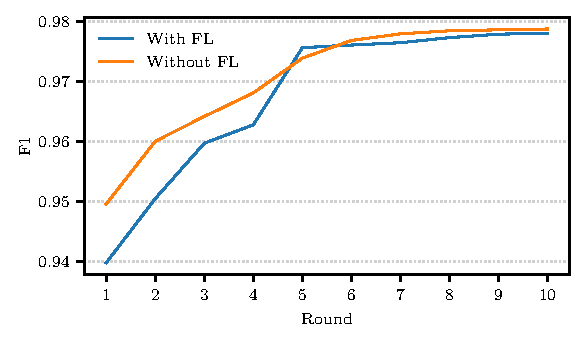
\includegraphics{figures/iid.pdf}
    \caption{Global model performance in IID.}
    \label{fig:iid}
\end{figure}


\subsection{Scenario 2: NIID Data from the Same Source\label{sec:app.demo.niid}}

The second scenario highlights the knowledge-sharing capabilities of \gls{fl}, as it can transfer characteristics of the data distribution between participants.
To illustrate this, after partitioning the data as in \Cref{sec:app.demo.iid}, we randomly drop two classes from each participant's train set.
This results in a \gls{niid} data distribution among participant, where each one has a different subset of classes.
\Cref{fig:niid} displays the results of this scenario, where \texttt{FedAvg} performs significantly better overall than having clients train locally.
However, the F1-score hides the fact that some participants can miss entire attack classes in the test set, rather than it being a global model issue.

Specifically, since clients have different subsets of classes, they might be unable to detect some intrusions that are not present in their training data.
For example, \Cref{tbl:niidclient} displays the \gls{dr} of the first client (\texttt{client\_0}) in our setup for each attack class, both in local and federated training, along with the number of samples of each class.
\texttt{client\_0} has no samples of the \texttt{Infiltration} and \texttt{DoS} classes, and therefore cannot detect them, \ie its \gls{dr} is either 0 or very low.
However, the global model is able to detect these classes, as other clients have samples of these classes in their training set.
We also see a slight decrease in performance for the other classes (\eg, 99.91 instead of 100 for \texttt{DDoS}) due to the aggregation process.
Note that the \texttt{Infiltration} being only detected at 20.11\% by the global model is the expected behavior on this dataset, as it is particularly difficult to detect (see the baseline results in \Cref{chap:assessment} for more details).

These results indicate that \gls{fl} can effectively share knowledge between participants, allowing them to detect attacks that are not present in their local training data.
This is a key feature of \gls{fl} in the context of intrusion detection.

\begin{figure}
    \centering
    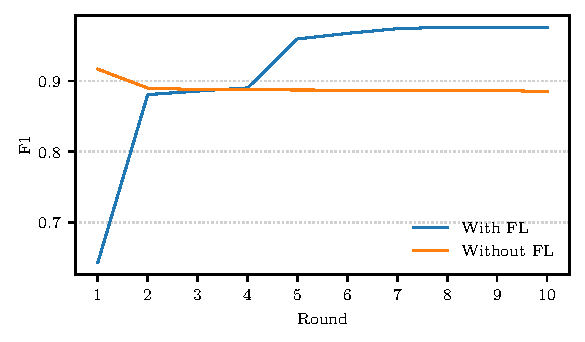
\includegraphics{figures/niid.pdf}
    \caption{Global model performance in NIID (same source).}
    \label{fig:niid}
\end{figure}

\begin{table}
    \centering
    \caption{Detection rate (DR) of \texttt{client\_0} in NIID settings. Rows where knowledge-sharing is visible are highlighted in gray.}
    \label{tbl:niidclient}
    \begin{tabular}{l|rrr}
        \toprule
        \textbf{Attack class} & \textbf{Samples} & \textbf{DR (local)} & \textbf{DR (federated)} \\
        \midrule
        DDoS & 176107 & 100 & 99.91 \\
        \rowcolor{lightgray} DoS & 0 & 2.43 & 98.57 \\
        Bot & 1513 & 100 & 99.94 \\
        Brute force & 1299 & 99.77 & 99.55 \\
        \rowcolor{lightgray} Infiltration & 0 & 0 & 20.11 \\
        Injection & 3 & 100 & 100 \\
        \bottomrule
    \end{tabular}
\end{table}



\subsection{Scenario 3: NIID Data from Different Sources\label{sec:app.demo.heterogeneous}}

While we highlight in \Cref{sec:app.demo.niid} that \gls{fl} can benefit from having different datasets per client, to the point where it can share knowledge between participants, the third scenario illustrates the limits of this assumption.
\Gls{cids} experiments in the literature often evaluate their approach with a scenario close to the ones presented in \Cref{sec:app.demo.iid,sec:app.demo.niid}, where one dataset is partitioned among participants.
However, in practice, participants will likely collect data from different networks, and therefore have different data distributions.

In this third scenario, we test \texttt{FedAvg} in this configuration, with each participant having a different dataset.
Thanks to the standardized feature set~(see \Cref{sec:app.demo.setup}), we can use the same model architecture for all participants, which is a requirement for \texttt{FedAvg}.
The class overlap between datasets is also not an issue in this use case, as we focus on binary-classification, which implies that all participants have benign and malicious samples.

The results presented in \Cref{fig:heterogeneous} confirm great performances overall when participants are trained locally. 
However, the global model's performance is highly impacted by the heterogeneity of the data distributions.
This is likely due to the fact that all participants converge to local minima that are too different from each other, and therefore the aggregation do not result in a suitable model for all participants.
Other approaches than \texttt{FedAvg} have been proposed to address this issue in \gls{ids} context, as the one by \textcite{popoola_FederatedDeepLearning_2021} for instance, who use \texttt{Fed+}~\cite{kundu_RobustnessPersonalizationFederated_2022a} as the aggregation strategy and present promising results in a similar scenario.

\begin{figure}
    \centering
    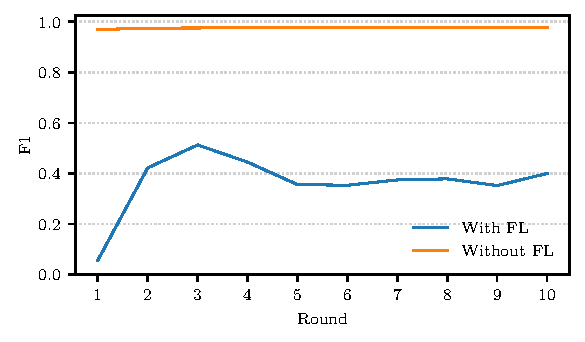
\includegraphics{figures/heterogeneous.pdf}
    \caption{Global model performance in NIID (different sources).}
    \label{fig:heterogeneous}
\end{figure}


\subsection{Scenario 4: Poisoning Attacks\label{sec:app.demo.poisoning}}

With the first three scenarios, we have highlighted how the heterogeneity between participants can impact the performance of \gls{fl}.
However, these scenarios assume that participants are honest and respect the protocol.
In this last scenario, we demonstrate how \gls{fl} can be vulnerable to malicious participants, whose goal is to degrade the performance of the global model.
To do so, we use a specific type data poisoning attacks (see \Cref{sec:bg.fl.threats}), where attackers flip the labels of samples in their training data to degrade the performance of the global model.
We use the same setup as in \Cref{sec:app.demo.iid}, with four participants and \gls{iid} partitioning.

In order to observe the impact in an extreme scenario, two of the four clients are instructed to perform a label flipping attack on their entire training set.
We can observe in local training (\Cref{fig:poisoning}) that participants identified as ``Attackers'' have a very low \gls{dr} on their test set, as they literally misclassify all of their testing samples.
The two benign participants, on the contrary, reproduce the results of \Cref{sec:app.demo.iid}, with a high \gls{dr} on their test set.

In \gls{fl} however, the global model is impacted by the malicious participants, as illustrated in \Cref{fig:poisoning}.
The participants cannot converge towards a stable global model, as the malicious participants' updates are too different from the others.
Due to the miss-classification introduced by the malicious participants, the global model's performance is degraded, and the F1-score oscillates between 0.1 and 0.2.
This is critically low, as it means that the aggregated model either misses a lot of attacks and misclassifies a lot of benign samples.
A more in-depth analysis of the impact of poisoning attacks on \gls{fl} is presented in \Cref{chap:assessment}.

\begin{figure}
    \centering
    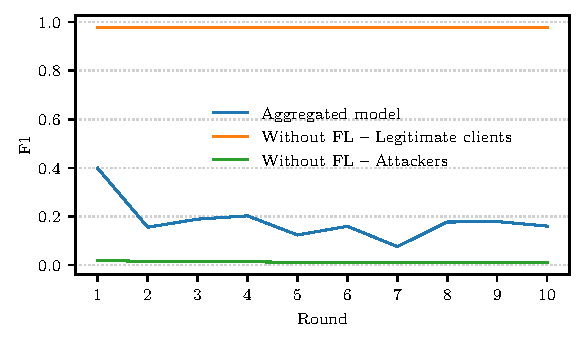
\includegraphics{figures/poisoning.pdf}
    \caption{Global model performance in poisoning attacks.}
    \label{fig:poisoning}
\end{figure}

%\section{}

% --------------------

\section{Conclusion and Takeways\label{sec:app.conclusion}}

In this chapter, we have presented a practical use case for \gls{fl} in the context of \glspl{cids}.
This use case will be used throughout the rest of the manuscript to illustrate the different contributions and results.
Based on this use case, we have also exposed some limitations of \glspl{fids}, notably in terms of data heterogeneity and susceptibility to poisoning attacks.
We will explore these limitations further in the next chapters: the impact of data heterogeneity in \Cref{chap:topologies}, and the impact of poisoning attacks in \Cref{chap:assessment}.
Finally, we will present some solutions to these limitations in \Cref{chap:radar} and \Cref{chap:future}.